%%%%%%%%%%%%%%%%%%%%%%%%%%%%%%%%%%%%%%%%%%%%%%%%%%%%%%%%%%%%%%%%%%%%%%%%%%%%%%%%%%%%%%%%%%%%%%%%%%%%%%%%%%%%
\subsection{Baseline}
%%%%%%%%%%%%%%%%%%%%%%%%%%%%%%%%%%%%%%%%%%%%%%%%%%%%%%%%%%%%%%%%%%%%%%%%%%%%%%%%%%%%%%%%%%%%%%%%%%%%%%%%%%%%
The first experiment done for a dataset is to train a classifier with data that is from the same domain as the test set.  In NORB, this is using the real photographs for training and in ShapeNet, it is the highest sample count Mitsuba rendered images. 
%To establish a baseline performance level we train our classifier on the NORB dataset using the ``real'' RGB image data. 
Note that for our experiments we use a single lighting condition for both test and training data to simplify experimental setup.  
%This reduces the test and training datasets to 4,050 images each. 
A synthetic g-buffer is constructed for each image in the training set at the target resolution.

This establishes a target classifier accuracy to be used for measuring the induced accuracy of using the training data created by the rendering methods used in this work. Next, we conduct multiple experiments by varying various rendering parameters and measuring their quantitative impact on classifier performance.  %See figure \ref{fig:norb-samples} for examples of the NORB images.

\edit{TO RESULTS: Training with the ``real'' NORB data yields a 95.01\% accuracy.}


%%%%%%%%%%%%%%%%%%%%%%%%%%%%%%%%%%%%%%%%%%%%%%%%%%%%%%%%%%%%%%%%%%%%%%%%%%%%%%%%%%%%%%%%%%%%%%%%%%%%%%%%%%%%
\subsection{No Shading - Albedo Only}
%%%%%%%%%%%%%%%%%%%%%%%%%%%%%%%%%%%%%%%%%%%%%%%%%%%%%%%%%%%%%%%%%%%%%%%%%%%%%%%%%%%%%%%%%%%%%%%%%%%%%%%%%%%%
To establish a baseline for synthetic performance we train with just the albedo map as input.  This is equivalent to an unshaded scene, and establishes what the classifier can learn without any shading information. See figure \ref{fig:GBUFFER_ALBEDO}.  
%%%%%%%%%%%%%%%%%%%%%%%%%%%%%%%%%%%%%%%%%%%%%%%%%%%%%%%%%%%%%%%%%%%%%%%%%%%%%%%%%%%%%%%%%%%%%%%%%%%%%%%%%%%%
\subsection{Shading Extracted from Rendering Through Learnable Spherical Harmonics}\label{sec:learned_sh}
%%%%%%%%%%%%%%%%%%%%%%%%%%%%%%%%%%%%%%%%%%%%%%%%%%%%%%%%%%%%%%%%%%%%%%%%%%%%%%%%%%%%%%%%%%%%%%%%%%%%%%%%%%%%
\begin{figure}[h!]
\centering
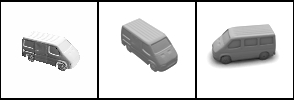
\includegraphics[width=1.0\columnwidth]{./assets/sh-comp-onerow.png}
\caption{Left: Learned SH. Middle: SH x Albedo. Right: SH x Albedo x Ambient Occlusion.}
\label{fig:SHComparison}
\end{figure}

\begin{figure}[h!]
\centering
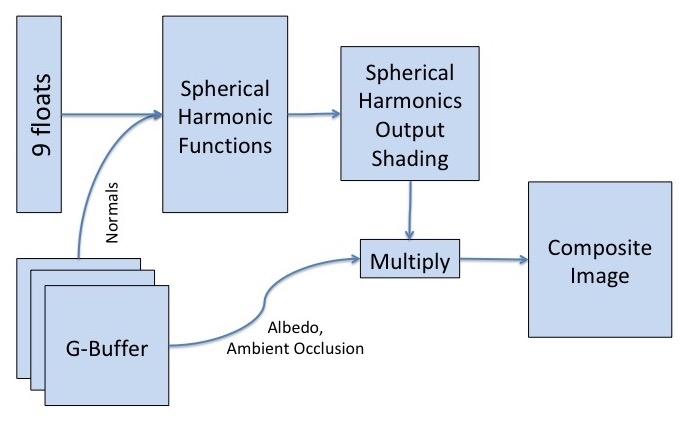
\includegraphics[width=1.0\columnwidth]{./assets/SH_model.jpg}
\caption{Spherical Harmonics network architecture.}
\label{fig:SHN}
\end{figure}
The next step beyond albedo-only rendering is shading without shadows. We chose to learn the shading given a full rendering target of the input g-buffer. This keeps the shading in the generated images approximately equal to the more sophisticated multi-bounce GI based images.  It allows for the testing of the impact of the presence of shadows in the synthesized images.
We accomplished this with a Spherical Harmonics (SH) module that enabled learning the 9 parameters to the 3 bands of functions.  These are enough bases to learn diffuse surfaces within a 99\% accuracy \cite{Shreiner:2013:OPG:2544032}. 


The input data to the SH module is the normal and albedo buffers.  The target is the full 128 sample GI render of the scene.  The SH module takes the normals as input and outputs an intensity.  \edit{That is then multiplied by the albedo and passed into an L1 loss function. For this experiment we chose L1 because given the output of the SH module was smooth and the number of learnable parameters was tiny we didn't need a complex loss function to get accurate results.} The loss is then backpropagated through the SH layer to adjust the shading. This is represented in figure \ref{fig:SHN}.

The result is a network that has learned the shading of the objects based upon the lighting in the target images.  The output also has the desired property of not having any shadows and allows us to test for shading based on surface normals.

For examples of the learned SH lighting see figure \ref{fig:SHComparison}.

\kris{PUT INTO DISCUSSION: The increase in accuracy gained by combining SH with albedo and AO shows that at least some form of shadows are important for classification.}


%%%%%%%%%%%%%%%%%%%%%%%%%%%%%%%%%%%%%%%%%%%%%%%%%%%%%%%%%%%%%%%%%%%%%%%%%%%%%%%%%%%%%%%%%%%%%%%%%%%%%%%%%%%%
\subsection{Two Bounce Mitsuba}\label{sec:2bounce}
%%%%%%%%%%%%%%%%%%%%%%%%%%%%%%%%%%%%%%%%%%%%%%%%%%%%%%%%%%%%%%%%%%%%%%%%%%%%%%%%%%%%%%%%%%%%%%%%%%%%%%%%%%%%

\begin{figure}[h!]
\centering
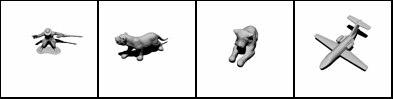
\includegraphics[width=1.0\columnwidth]{./assets/2bounce_small.png}
\caption{Two Bounce Rendering.  Note that it is the equivalent to a shadow mapped scene and differs from the AO composited scenes by the sharpness of the shadows. This is due to the scene using a single directional light.}
\label{fig:2BOUNCE}
\end{figure}
% TODO: this paragraph bounces between past and present tense, reads kind of weird
Now that we have seen that an approximate shadow (Ambient Occlusion) aids classification \tompson{Rephrase this if you're moving it into the discussion section (because they haven't seen any results yet)...}, we add shadows to the synthetic dataset. However, we don't want inter-reflections and global illumination, as we test that separately \tompson{Rephrase: Just say that you want to measure the impact of inter-reflections and global illumination but with some shadow detail, and so you also include an experiment where you restrict the number of bounces to 2.}.  This can be achieved in Mitsuba by limiting how many bounces the rays take during simulation.  We only allow the rays fired through the screen to hit an object, bounce, and see if it hits a light source.  There are no secondary bounces to allow indirect lighting to illuminate the object. We also choose \tompson{past-tense is chose?} to use a single directional light to create very hard shadows.  This will allow us to contrast the performance of hard shadows and soft shadows which are both present in the real dataset.  This is also a good approximation of what a video game engine might produce and can be used as a proxy for video game engine generated synthetic data \tompson{Is this true? Most engines these days have some form of (crappy) GI.}.  See figure \ref{fig:2BOUNCE} for examples of this rendering method.  \tompson{Move this into a discussion section to be consistent.} The resulting performance from training with this data was very similar to SH composited with albedo and AO \tompson{What is A0? First use of this term.}.  It yields an accuracy of 55.78\%.  A possible explanation could be that the real data has one sharp shadow from an overhead light and a soft shadow from another. Additionally, ambient occlusion is a good approximation of the dominant light source in the scene which is large with uniform brightness and occupies a large part of the hemisphere surrounding the object.


%%%%%%%%%%%%%%%%%%%%%%%%%%%%%%%%%%%%%%%%%%%%%%%%%%%%%%%%%%%%%%%%%%%%%%%%%%%%%%%%%%%%%%%%%%%%%%%%%%%%%%%%%%%%
\subsection{Varying Sample Count in the Mitsuba Path Tracer}
%%%%%%%%%%%%%%%%%%%%%%%%%%%%%%%%%%%%%%%%%%%%%%%%%%%%%%%%%%%%%%%%%%%%%%%%%%%%%%%%%%%%%%%%%%%%%%%%%%%%%%%%%%%%

\tompson{To make this seem less like a collection of unrelated experiments, I suggest you rename your subsubsection headings so that there is a consistent progression. I would expect: Albedo Rendering (no shading), Learned-Diffuse Rendering (shading with no shadows), Single-Bounce Rendering (shading with hard shadows), Multi-Bounce Rendering (shading with soft shadows).  These section headings will make the store a lot cleaner...}

\begin{table*}[]
\centering
\begin{tabular}{|l|r|r|r|r|}
\hline
\multicolumn{1}{|c|}{\textbf{Input}}
& \multicolumn{1}{c|}{\textbf{1 Sample}}
& \multicolumn{1}{c|}{\textbf{4 Sample}}
& \multicolumn{1}{c|}{\textbf{128 Sample}}
& \multicolumn{1}{c|}{\textbf{$\Delta$ vs Real}} \\ \hline
Mitsuba		& 64.44\%	& 73.13\%	& 74.74\%	& 20.27 / 78.67\% \\
Denoised	& 71.48\%	& 73.56\%	& N/A 		& 21.45 / 77.42\%	\\
Single GAN	& 72.84\%	& 77.65\% 	& 75.26\%	& \textbf{17.36 / 81.73\%}	\\
Multiple GAN& 85.23\%	& 84.37\% 	& 87.33\% 	& \textbf{7.68 / 91.92\%}		\\ \hline
\multicolumn{5}{|c|}{\textbf{Performance of GI Rendered Refined Images}}	\\ \hline
\end{tabular}
\caption{Comparison of GI Rendered Refined Image Performance. The GAN output refers to if only one GAN was used to refine the dataset or if the dataset was expanded by multiple GANs\tompson{What GAN output? This is the first time your mentioning GANs. Never, ever, ever, ever (times infinity + 1) show results for a term, model, experiment, etc without first describing it. For this reason, I would move this table WAY down a few pages on.}. $\Delta$ \tompson{IMO, I find this notation confusing. "Performance loss" would be a better column heading.} vs Real has two numbers \tompson{Yes, this is confusing. Pick one of these to show (it's redundant to have both). Simple is better.}. The left is the difference in accuracy from the best result of each method compared to using real data (Real achieved \textbf{95.01\%}). See section \ref{sec:gans} for further details.  The second number is the percentage of the real data trained classifier's accuracy that the method achieves.  100\% would mean that the method would have achieved 95.01\% accuracy when training a classifier. See section \ref{sec:multigans} for more details \tompson{Rule of thumb: a reader should have already read all information they need to understand your results}. Bold values represent values that are better than the accuracy of the best quality GI rendering (128 Sample Mitsuba) \tompson{Remove the bold highlighting.}. Data augmentation was used for the Mitsuba experiments. \tompson{caption is too long. Move some content into body text.}}
\label{tblallrefined}
\end{table*}

\begin{table*}[]
\centering
\begin{tabular}{|l|r|r|r|}
\hline
\multicolumn{1}{|c|}{\textbf{Input}}
& \multicolumn{1}{c|}{\textbf{10 Sample}}
& \multicolumn{1}{c|}{\textbf{32 Sample}}
%& \multicolumn{1}{c|}{\textbf{128 Sample}}
& \multicolumn{1}{c|}{\textbf{$\Delta$ vs Real}} \\ \hline
Mitsuba		& 81.68\%	& 82.30\%	& 1.69 / 97.99\% \\
Denoised	& 78.06\%	& 79.12\%	& 3.08 / 96.25\%	\\
Single GAN	& 83.48\%	& 83.59\%	& \textbf{0.40 / 99.52\%}	\\
Multiple GAN& 86.48\%	& 86.65\% 	& \textbf{-2.66 / 103.17\%}		\\ \hline
\multicolumn{4}{|c|}{\textbf{Performance of GI Rendered Refined Images}}	\\ \hline
\end{tabular}
\caption{Scores using the Shapenet dataset. Data augmentation was not used for the experiments listed above.}
\label{tblallrefined}
\end{table*}

%\begin{figure}[h!]
\centering
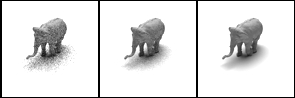
\includegraphics[width=1.0\columnwidth]{./assets/mitsuba-onerow.png}
\caption{
Mitsuba renders at different sample counts. Left: 1 sample per pixel.  Middle: 4.  Right: 128.}
\label{fig:differentsamplesraw}
\end{figure}
\begin{comment}
\begin{figure}[h!]
\centering
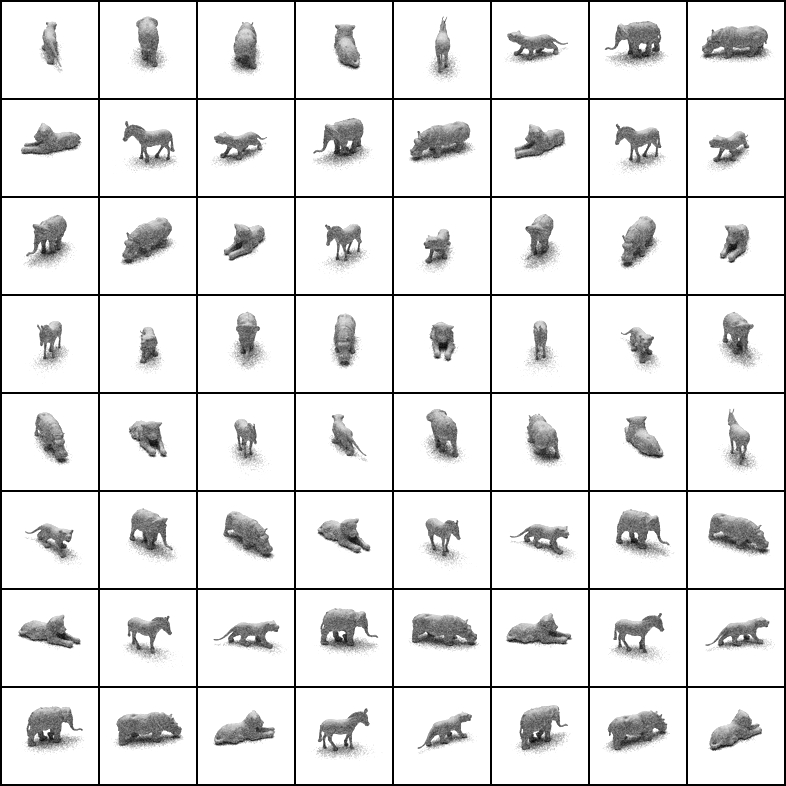
\includegraphics[trim={0 0 392px 687px},clip,width=1.0\textwidth]{./assets/traindata_1_sample.jpg}
\caption{Sample crop 1.}
\label{fig:crop1}
\end{figure}
\begin{figure}[h!]
\centering
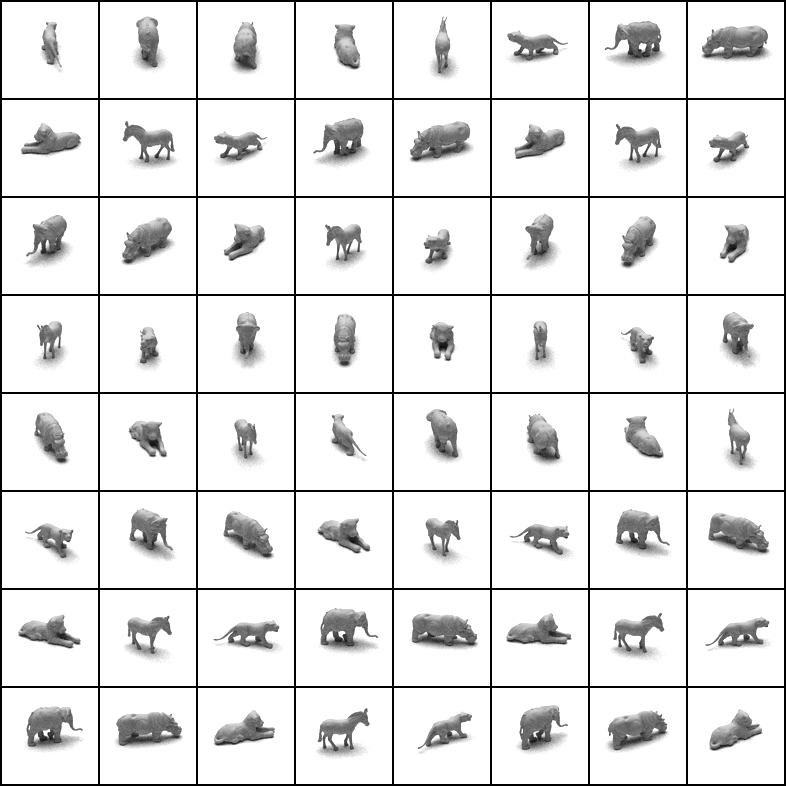
\includegraphics[trim={0 0 392px 687px},clip,width=1.0\textwidth]{./assets/traindata_4_sample.jpg}
\caption{Sample crop 4.}
\label{fig:crop4}
\end{figure}
\begin{figure}[h!]
\centering
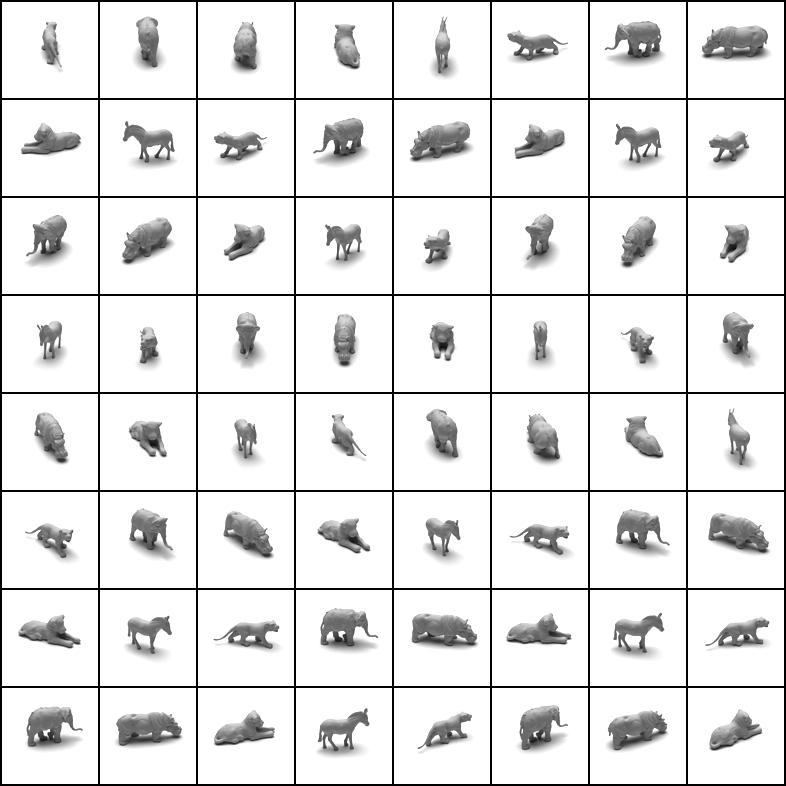
\includegraphics[trim={0 0 392px 687px},clip,width=1.0\textwidth]{./assets/traindata_target_128_sample.jpg}
\caption{Sample crop 128.}
\label{fig:crop128}
\end{figure}
\end{comment}


The last rendering feature that we add to achieve the most realism is allowing light to bounce inside the environment, reflecting off surfaces and onto other objects in the scene.  Multiple bounces soften the shadows and allow light to come from below the object by reflecting off the ground plane. \tompson{And other stuff! Volumetric fog, mirrors, ambient occlusion, etc...}

A global illumination (GI) renderer creates images by firing rays through each pixel and checks for intersections with surfaces in the scene \tompson{Too general a statement. Not all GI renderers are ray marching/tracing! Rephrase as, "For our GI experiments we will use Mitsuba, a ray tracing GI rendering engine, which renders by sampling rays, ......" Or something like that. But in general though, I'm a little worried that you're over explaining stuff. The confusing thing is that you've already talked about number of bounces in the previous section, and so all you should need to say here is that you let the number be > 1. You might want to consider moving a condensed version of your ray-tracer explanation earlier in the experimental setup when you first mention Mitsuba.}.  If it hits anything, it then fires many more rays emanating from the hit point and determines, inside a certain number of bounces, if the ray eventually hits a source of light.  It is important to realize that it takes many samples per bounce to accurately determine all of the incoming light arriving at a point upon an object's surface.
%Random sampling plays a heavy part in allowing the calculations to be efficient. 
However, if not enough samples are used it GI introduces noise into the final output. This is especially true for scenes composed of shiny surfaces and small bright light sources which induce light intensities along surfaces that can change very quickly. \tompson{Yeah, for sure this feels like thesis-filler. It's WAY too verbose and is borderline insulting the intelligence of your readers...  I mean, we know they're all stupid, but we don't have to call it out ;-)}

We are fortunate that our scenes only \tompson{"our" here and in the next sentence is too possessive. The NORB scenes are not yours.} involve surfaces that are diffuse and light sources that are relatively large compared to the illuminated objects.  Therefore it takes fewer samples to resolve the lighting for our images, as the intensity of reflected light varies slowly across a diffuse surface.  However, we found we needed at least 128 samples per pixel to reduce the noise to be imperceptible \tompson{change imperceptible to either use a precise measure (SNR measures for instance) or something even more vague "to be acceptable". "imperceptible" implies that you just tweaked values until you thought it looked good.}. High sample count is a known problem with GI renderers, and is a major factor in the high computational cost per image.  For complex scenes with certain lighting and materials, it can take hours to generate an image.  Even in our simple \tompson{avoid "simple"} scenes, it still took over a minute per image at 768x768 and 128 samples per pixel, while using one or four samples per pixel took only a few seconds a frame.

%Given that the full sample images are expensive to compute, can you use the noisy images? Is the noise in the image a problem for a convnet based classifier?  \footnote{This question was also asked by \cite{DBLP:journals/corr/VeeravasarapuRR16}. See Related work section}. To answer this question, 
We generated datasets using just one per pixel and four samples per pixel \tompson{huh? why did you mention 128 then?}. We then used them to directly train a classifier.  We learned that the classifier can handle some noise without a performance penalty,  but too much noise hurts performance enough to negate the fact that a GI renderer is being used.  The baseline comparison is the 128 ``noiseless'' image \tompson{ahhhhhh. now I get it. Rephrase as "we generated datasets using 1, 4 and 128 samples per pixel, where we consider 128 samples to be a good approximation of a noiseless (ideal) render.}, which achieves a performance of 74.84\%.  The 4-sample image is close in performance but also does not have much noise.  It gets an accuracy of 72.89\%, which is quite close to 128 samples while being 32 times less computation.  \tompson{Again, move performance numbers somewhere else? or at this point just be consistent.} The single sample image only achieves an accuracy of 57.21\%, which is significantly worse and is in the same order of accuracy as much cheaper rendering methods. However, the single sample per pixel image has a significant amount of noise \tompson{You didn't measure it so how do you know it's significant. It's only reasonable to say that the trend is expected due to the increase in noise (not that YOU think it's value is significant).}.  The difference between the 1 and 4 sample images is most apparent at the edges \tompson{Edges of what? The image? The geometry? The Shadows? Be specific.}. Four samples seems to be enough to have resolvable edges while only 1 sample was insufficient to define a border between shadow and unshadowed regions. See figure \ref{fig:differentsamplesraw} to see the difference in image quality based upon sample count. 
%Mitsuba is a free open source path tracer that allows for the control of how many bounces a light can take before it no longer is simulated and it allows for how many samples are taken per pixel.\\

%%%%%%%%%%%%%%%%%%%%%%%%%%%%%%%%%%%%%%%%%%%%%%%%%%%%%%%%%%%%%%%%%%%%%%%%%%%%%%%%%%%%%%%%%%%%%%%%%%%%%%%%%%%%
\subsection{Train on Denoised Images} \label{denoising}
%%%%%%%%%%%%%%%%%%%%%%%%%%%%%%%%%%%%%%%%%%%%%%%%%%%%%%%%%%%%%%%%%%%%%%%%%%%%%%%%%%%%%%%%%%%%%%%%%%%%%%%%%%%%
%Remembering that GI renderers are computationally expensive, we wanted to try techniques that would lower the render time. We wanted to see if we can get away with allowing the GI renderer to use fewer samples per pixel, and as a result, spend much less time computing images while maintaining the same performance from the dataset. 
Knowing that noisy images are still useful for training, we leverage the information in them to create a new image that performs better. Utilizing noisy rendered images and their corresponding ``real'' RGB version, we trained a generative model to denoise the dataset images before training. To do so we use a simplified version of the denoising auto-encoder with skip connections network proposed by \cite{Chaitanya:2017:IRM:3072959.3073601}, where we do not include the recurrent portion of their proposed architecture since we train using static images rather than animated sequences as in \cite{Chaitanya:2017:IRM:3072959.3073601}. The resultant network is shown in figure \ref{fig:denoise} \tompson{Go through the entire paper and make sure you use \text{Figure~\ref{}} to reference figures... (not the Capital and tilde).}. 
\begin{figure}[h!]
\centering
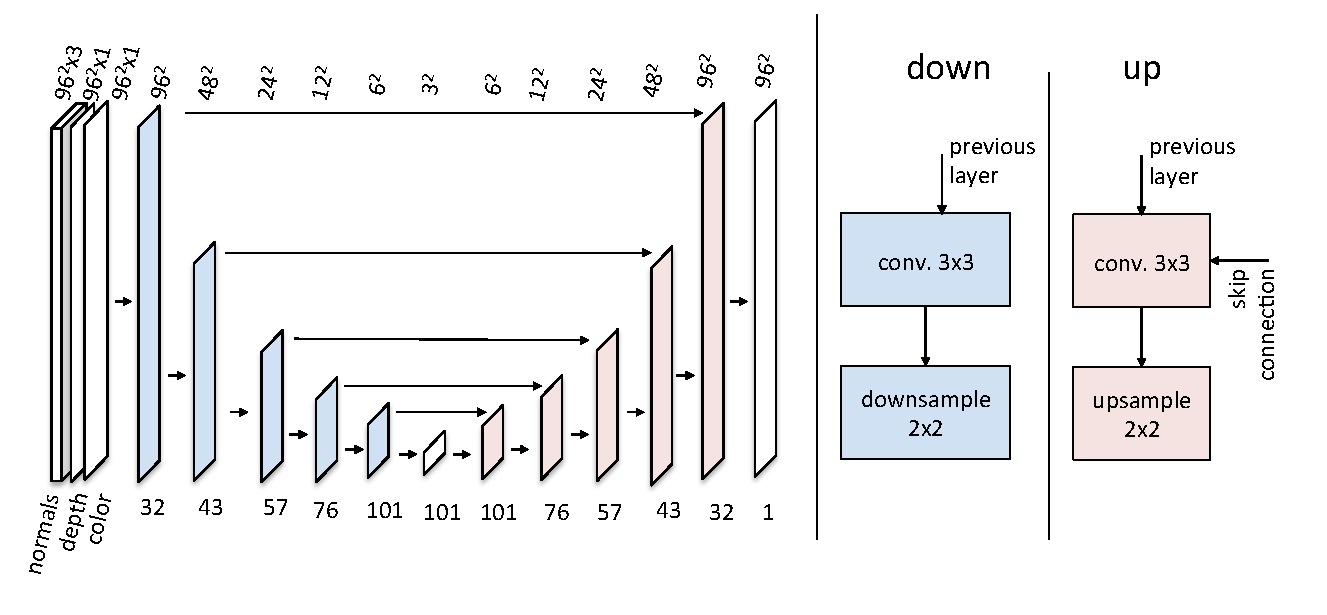
\includegraphics[width=1.0\columnwidth]{./assets/denoiser_diagram.pdf}
\caption{Architecture of Denoising Model}
\label{fig:denoise}
\end{figure}

The loss function we used for training the denouncing generative model is Structured Similarity (SSIM)\cite{Wang04imagequality}. SSIM is typically used for image compression measurement, but also has been shown to be a good loss function for image comparison. The function for SSIM is given by
$$SSIM(p)=\frac{2\mu_x\mu_y + C_1}{\mu_x^2+\mu_y^2+C_1}\cdot\frac{2\sigma_{xy}+C_2}{\sigma_x^2+\sigma_y^2+C_2}$$
where $\mu$ is the mean of the pixel $p$ computed with a Gaussian filter, $\sigma^2$ is the variance and $\sigma_{xy}$ is the covariance. SSIM can be thought of as having a combination of three different measures: a luminance comparison for an approximate average difference in brightness,  a contrast comparison which measures a difference in brightness variance, and finally a structure comparison which uses a ration between the covariance and variance of the two images.  See \cite{DBLP:journals/corr/ZhangSYSLJF16} and \cite{DBLP:journals/corr/ZhaoGFK15} for details.

Denoising 1-sample images boosted accuracy from 57.21\% to 71.48\%, which is close to both 4 and 128 samples in performance while being much more accurate than other inexpensive rendering methods. Also, it is important to note that the rendering cost is two orders of magnitude lower than using the full sample count. 4 sample images, due to their low noise, only show a slight boost in performance: 72.89\% to 73.56\%.  The unadulterated \tompson{This is not a thing. It is not in the vernacular of academic papers.} 128 sample image achieved 74.84\%, which is only slightly better than the denoised low sample images.  Given that the denoising process takes milliseconds on a GPU \footnote{NVIDIA GeForce Titan X with 12GB or VRAM}, the cost of denoising is insignificant compared to taking more samples in a GI renderer \tompson{State this FIRST before any other results. This is the important take away from this paragraph.}.  See figure \ref{fig:differentsamplesraw} to see direct comparisons between images generated with different sample counts.

All of the results are listed in Table \ref{tblallrefined}.

\tompson{Why are there 2 tables with this label?!}


\begin{comment}
\begin{table}[]
\centering
\label{tbldenoiseperf}
\begin{tabular}{|l|c|c|}
\hline
Samples        & 1             & 4             \\ \hline
Accuracy       & 71.48\%       & 73.56\%       \\ \hline
\multicolumn{3}{|c|}{Denoised Images Accuracy} \\ \hline
\end{tabular}
\caption{Performance of training on denoised images}
\end{table}
\end{comment}